%%%%%%%%%%%%%%%%%%%%%%%%%%%%%%%%%%%%%%%%%
% University Assignment Title Page 
% LaTeX Template
% Version 1.0 (27/12/12)
%
% This template has been downloaded from:
% http://www.LaTeXTemplates.com
%
% Original author:
% WikiBooks (http://en.wikibooks.org/wiki/LaTeX/Title_Creation)
%
% License:
% CC BY-NC-SA 3.0 (http://creativecommons.org/licenses/by-nc-sa/3.0/)
% 
% Instructions for using this template:
% This title page is capable of being compiled as is. This is not useful for 
% including it in another document. To do this, you have two options: 
%
% 1) Copy/paste everything between \begin{document} and \end{document} 
% starting at \begin{titlepage} and paste this into another LaTeX file where you 
% want your title page.
% OR
% 2) Remove everything outside the \begin{titlepage} and \end{titlepage} and 
% move this file to the same directory as the LaTeX file you wish to add it to. 
% Then add \input{./title_page_1.tex} to your LaTeX file where you want your
% title page.
%
%%%%%%%%%%%%%%%%%%%%%%%%%%%%%%%%%%%%%%%%%
%\title{Title page with logo}
%----------------------------------------------------------------------------------------
%	PACKAGES AND OTHER DOCUMENT CONFIGURATIONS
%----------------------------------------------------------------------------------------

\documentclass[12pt]{article}
\usepackage[english]{babel}
\usepackage[utf8x]{inputenc}
\usepackage{amsmath}
\usepackage{graphicx}
\usepackage[colorinlistoftodos]{todonotes}
\usepackage{hyperref}
\usepackage{listings}
\usepackage{appendix}
\usepackage{tabularx}
\usepackage{adjustbox}
\usepackage{multirow}
\usepackage{caption}
\usepackage{subcaption}


\begin{document}

\begin{titlepage}

\newcommand{\HRule}{\rule{\linewidth}{0.5mm}} % Defines a new command for the horizontal lines, change thickness here

\center % Center everything on the page
 
%----------------------------------------------------------------------------------------
%	HEADING SECTIONS
%----------------------------------------------------------------------------------------

\textsc{\LARGE University of Edinburgh}\\[1.5cm] % Name of your university/college
\textsc{\Large Programming Skills}\\[0.5cm] % Major heading such as course name
\textsc{\large Performance Testing Coursework}\\[0.5cm] % Minor heading such as course title

%----------------------------------------------------------------------------------------
%	TITLE SECTION
%----------------------------------------------------------------------------------------

\HRule \\[0.4cm]
{ \huge \bfseries Performance Report}\\[0.4cm] % Title of your document
\HRule \\[1.5cm]
 
%----------------------------------------------------------------------------------------
%	AUTHOR SECTION
%----------------------------------------------------------------------------------------



% If you don't want a supervisor, uncomment the two lines below and remove the section above
\Large \emph{Author:}\\
\textsc{Jack Frankland}\\[3cm] % Your name

%----------------------------------------------------------------------------------------
%	DATE SECTION
%----------------------------------------------------------------------------------------

{\large \today}\\[2cm] % Date, change the \today to a set date if you want to be precise

%----------------------------------------------------------------------------------------
%	LOGO SECTION
%----------------------------------------------------------------------------------------


\includegraphics[width=3cm, height=3cm]{logo.png}\\[3cm] % Include a department/university logo - this will require the graphicx package
 
%----------------------------------------------------------------------------------------

\vfill % Fill the rest of the page with whitespace

\end{titlepage}

\begin{abstract}
This report provides the results and analysis of various performance tests which were carried out on the 2D Predator-Prey model that was written for the first coursework. A range of different tests are used to evaluate the program and in each case the tests results are analyzed and interpreted. A conclusion is then reached about the overall quality of the program in terms of performance. 
\end{abstract}
\listoffigures
\listoftables
\tableofcontents

\section{Introduction}
\label{sec:introduction}
 

\section{Performance Tests and Analysis}
\label{sec:perf}


\subsection{Effects of Compiler Optimization Flags}
\label{subsec:opflags}
In this section we will investigate the performance effects of using different compilers with different optimization flags. To implement these tests we use a single $1000\times1000$ landscape given in \ref{fig:OptLandscape} which consists of two large land masses separated by a river of water. This landscape was chosen since it is large enough and generic enough to provide results that could be scaled for any realistic landscape. The input parameters for all tests in this section were fixed as:
\begin{itemize}
	\item Birthrate of prey 0.08
	\item Predation rate at which predators eat prey 0.04
	\item Birth rate of predators per one prey eaten 0.02
	\item Predator mortality rate 0.06
	\item Diffusion rate of prey 0.2
	\item Diffusion rate of predators 0.2
	\item Size of time step 0.4
	\item Number of time steps between output of plain .pnm file 10
\end{itemize}
\begin{figure}
\label{fig:OptLandscape}
\centering
\frame{
\includegraphics[scale=0.2]{OpTestLandscape.png}}
\caption{ $1000\times1000$ Test Landscape for optimization flags.}
\end{figure}

In order to get an accurate figure on the run time of the code under each compilation flag we initially planned to run the tests on the a single core on a Cirrus back end node. Because the traffic to Cirrus is fairly consistent, due to the fact is in constant use, this allows us to make performance measurements we know are reconstructible, and hence we can compare the run times with a good degree of confidence in their relative values. However, after some initial testing it was clear the code ran roughly 4-5 times faster on the cp-lab than it did on Cirrus. Further to this, we found that submitting several jobs to the Cirrus queue had the effect of slowing each job down by an amount proportional to the number of jobs submitted. The reason for this is not entirely clear; one possibility is that the different jobs were competing for memory on the front end node during output. This issue in particular made testing on Cirrus infeasible, since the run times were over ten minutes, and the jobs needed to be submitted one at a time, the total runtime would have been too large to get any results. Instead we decided to use the cp-lab, since the run times were faster we were able to submit jobs individually and since the cp-lab is in use most of the time we can assume our results accurately represent a standard job runtime. We ran 6 tests for each compiler flag and calculated the mean and standard error using equations \ref{eqn:std} and \ref{eqn:stderr}.



\begin{table}[!h]
\label{table:optimizationCPlab}
\begin{center}
\begin{adjustbox}{width=\textwidth,totalheight=\textheight,keepaspectratio}
\begin{tabular}{| c | c | c | c | c | c | c |}
\hline
\textbf{Compiler} & \multicolumn{6}{| c |}{\textbf{Run Time(s)}}  \\ 
\cline{2-7}
& \textbf{O0} & \textbf{O1} & \textbf{O2} & \textbf{O3} & \textbf{Ofast} & \textbf{Os} \\
\hline
gcc & $249.002 \pm 0.765$ & $181.647 \pm 0.571$ & $172.332 \pm 0.912$ & $174.978 \pm 0.777$ & $177.254 \pm
1.127$ & $190.362 \pm 0.496$\\ \hline
\end{tabular}
\end{adjustbox}
\end{center}
\caption{Run times for the sample $1000\times1000$ grid running on the cp-lab.}
\end{table}

From these results it is clear that under the gcc compiler the code runs fastest when compiled under the $\mathcal{O}2$ flag. This is slightly unexpected since one would expect the code to run fastest when compiled under the $\mathcal{O}3$ or $\mathcal{O}fast$ flags, however it is fairly common for different programs to run faster under different compiler flags due to the different optimisations the various compiler flags employ, and the content of the code itself.\\


We were interested in how well the program would perform under a completely different compiler, which is one of the reason we initially chose to use Cirrus. However, due to the fact the the cp-lab only has the gnu gcc compiler installed this meant using a different machine to compile the code. We chose to carry out these extra experiments on a Cirrus back end node and a Macbook to see how they would compare. Due to the long runtime for each test we were only able to carry out one test in each case and have not performed any statistical averages. 

\begin{table}[!h]
\label{table:optimizationMyComp}
\begin{center}
\begin{adjustbox}{width=\textwidth,totalheight=\textheight,keepaspectratio}
\begin{tabular}{| c | c | c | c | c | c | c |}
\hline
\textbf{Compiler} & \multicolumn{6}{| c |}{\textbf{Run Time(s)}}  \\ 
\cline{2-7}
& \textbf{O0} & \textbf{O1} & \textbf{O2} & \textbf{O3} & \textbf{Ofast} & \textbf{Os} \\
\hline
clang & 529.025 & 457.535 & 395.897 & 415.884 & 383.270 & 399.656 \\ \hline
intel & 552.608 & 378.542 & 373.768 & 361.429 & 687.909 & 395.915 \\ \hline
\end{tabular}
\end{adjustbox}
\end{center}
\caption{Run times for the sample $1000\times1000$ grid running on mid 2014 Macbook Pro with 2.8GHz Intel i5 processor with 8 GB 1600 MHz DDR3.}
\end{table}

\begin{table}[!h]
\label{table:optimizationCirrus}
\begin{center}
\begin{adjustbox}{width=\textwidth,totalheight=\textheight,keepaspectratio}
\begin{tabular}{| c | c | c | c | c | c | c |}
\hline
\textbf{Compiler} & \multicolumn{6}{| c |}{\textbf{Run Time(s)}}  \\ 
\cline{2-7}
& \textbf{O0} & \textbf{O1} & \textbf{O2} & \textbf{O3} & \textbf{Ofast} & \textbf{Os} \\
\hline
gcc & 800.220 & 723.293 & 724.042 & 698.490	 & 698.005 & 734.928 \\ \hline
intel & 871.976 & 751.004 & 728.728  &  &  & \\ \hline
\end{tabular}
\end{adjustbox}
\end{center}
\caption{Run times for the sample $1000\times1000$ grid running on Cirrus back end node with 1 cpu.}
\end{table}







\subsection{Main Sources of Overhead}
\label{subsec:overhead}
In order to identify the main sources of overhead in our program we used the Gnu gprof tool. The code was compiled under the gcc compiler with optimisation flags -O0 and without the debug flag -g. This is because compiling with optimizations turned on can lead to inlining of functions, which in turn causes them to disappear from the profiling tables, however since different compilers and different flags may inline different functions in different places, the profiling data would be specific to the compiler case, and not a general profile of the code. By compiling with -O0 we can identify overheads that will be common to all compilers for the -O0 (no optimizations) optimization level. The input parameters and landscape are the same as in section \ref{subsec:opflags}. Since they are extensive and rather verbose we have included the first pages only since they contain the functions with the largest overheads.

\begin{figure}
\label{fig:FlatP}
\centering
\frame{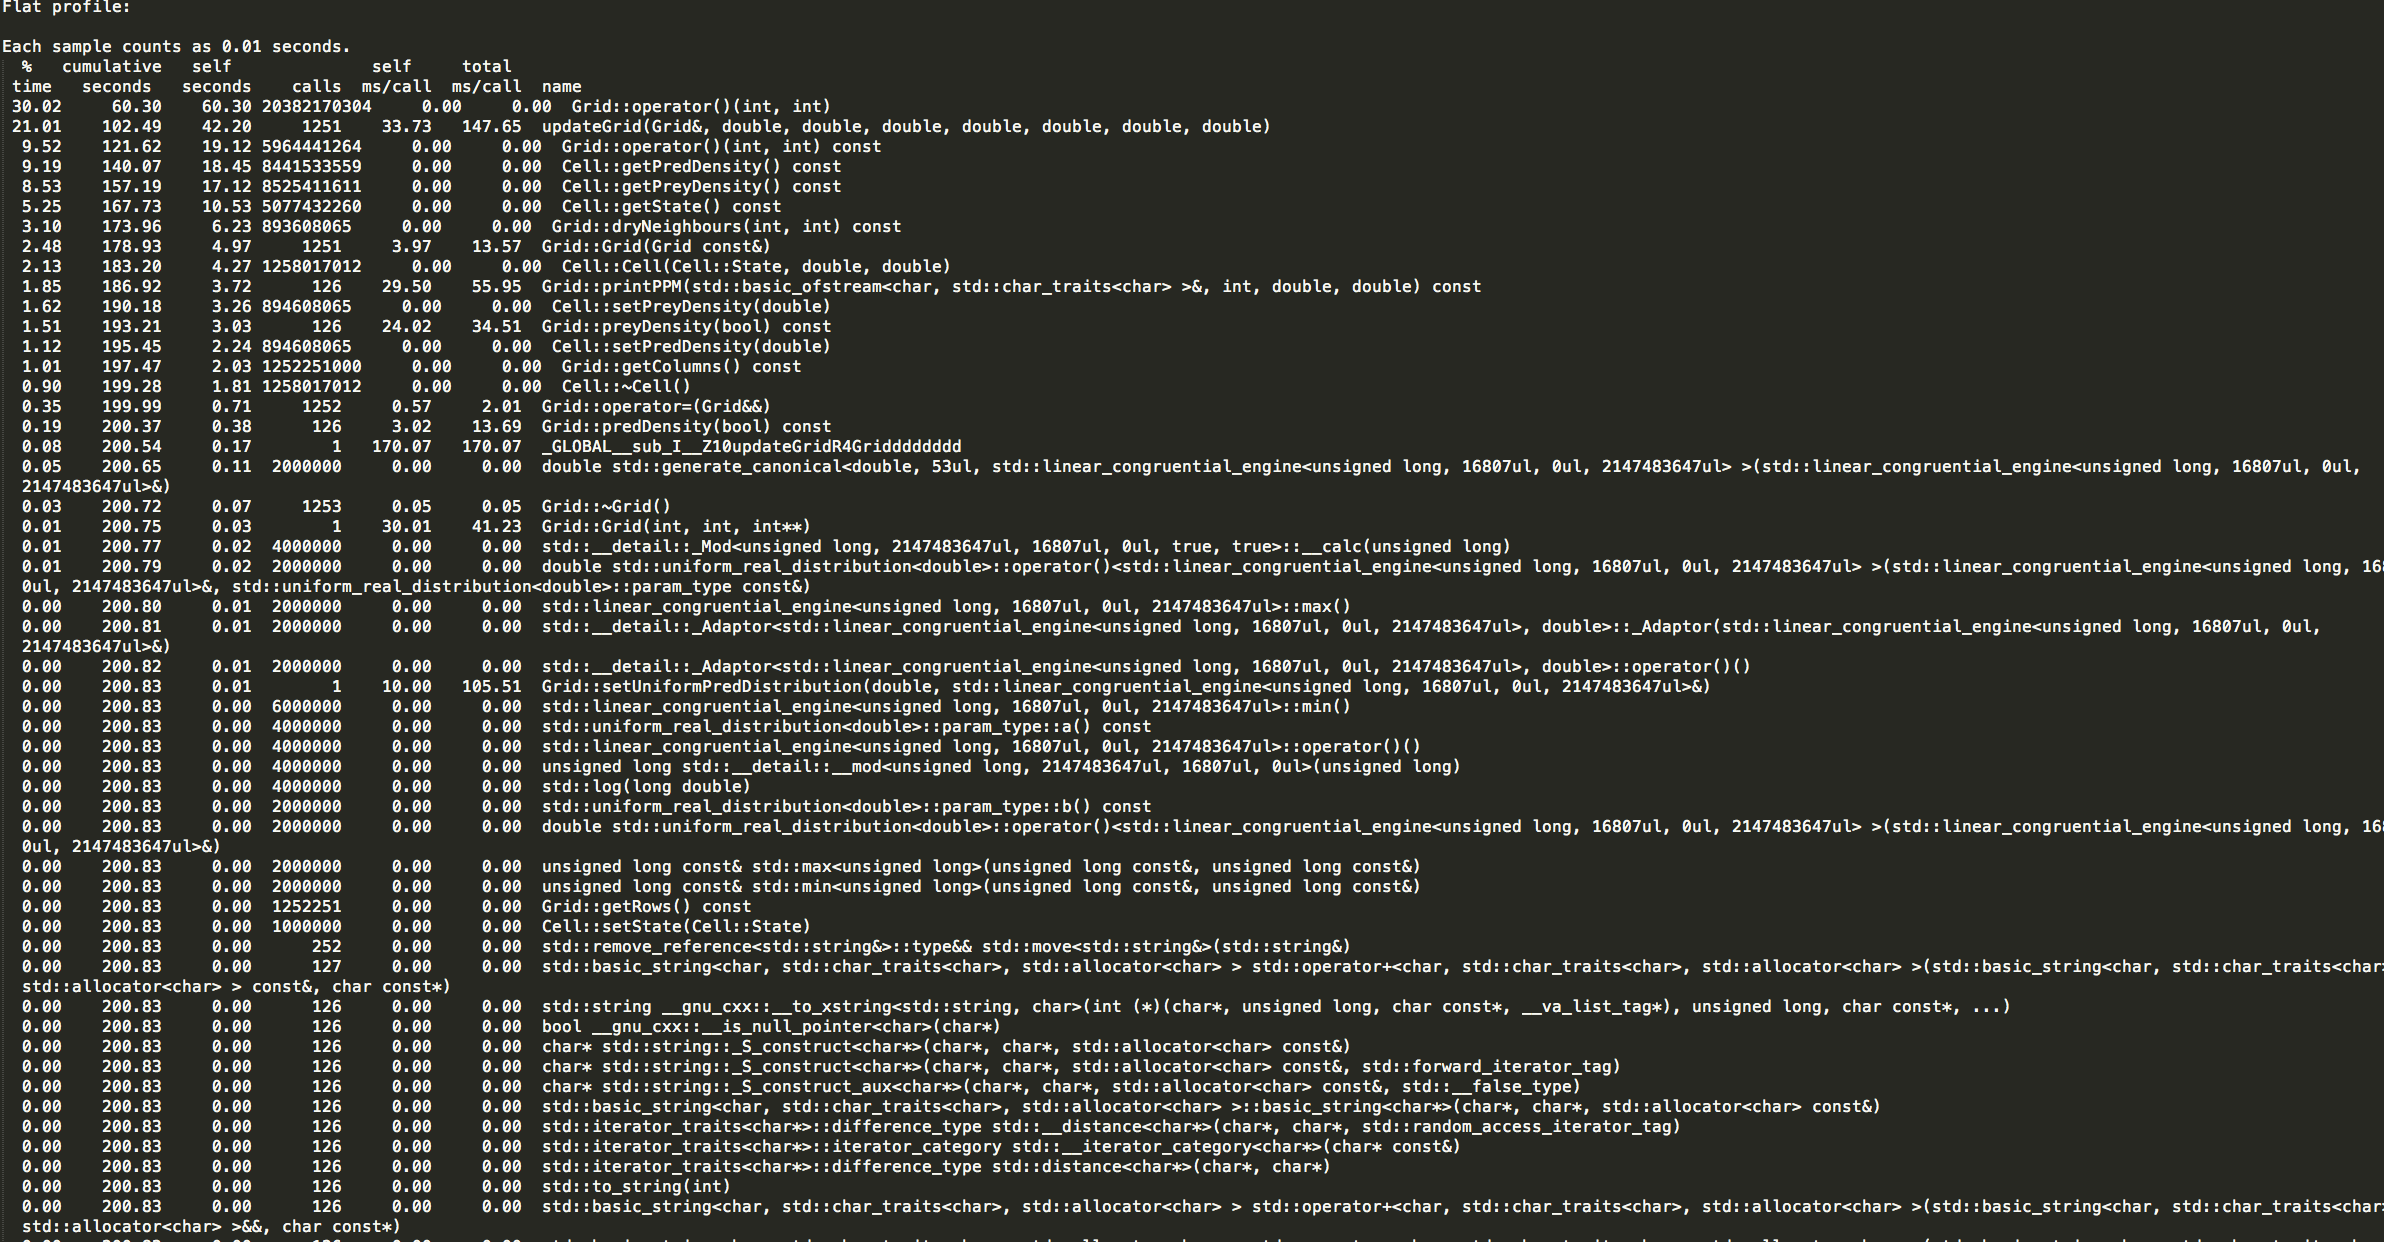
\includegraphics[scale=0.3]{Flat-Profile.png}}
\caption{Flat profile page 1. for Gnu gprof profiler.}
\end{figure}

\begin{figure}
\label{fig:CallG}
\centering
\frame{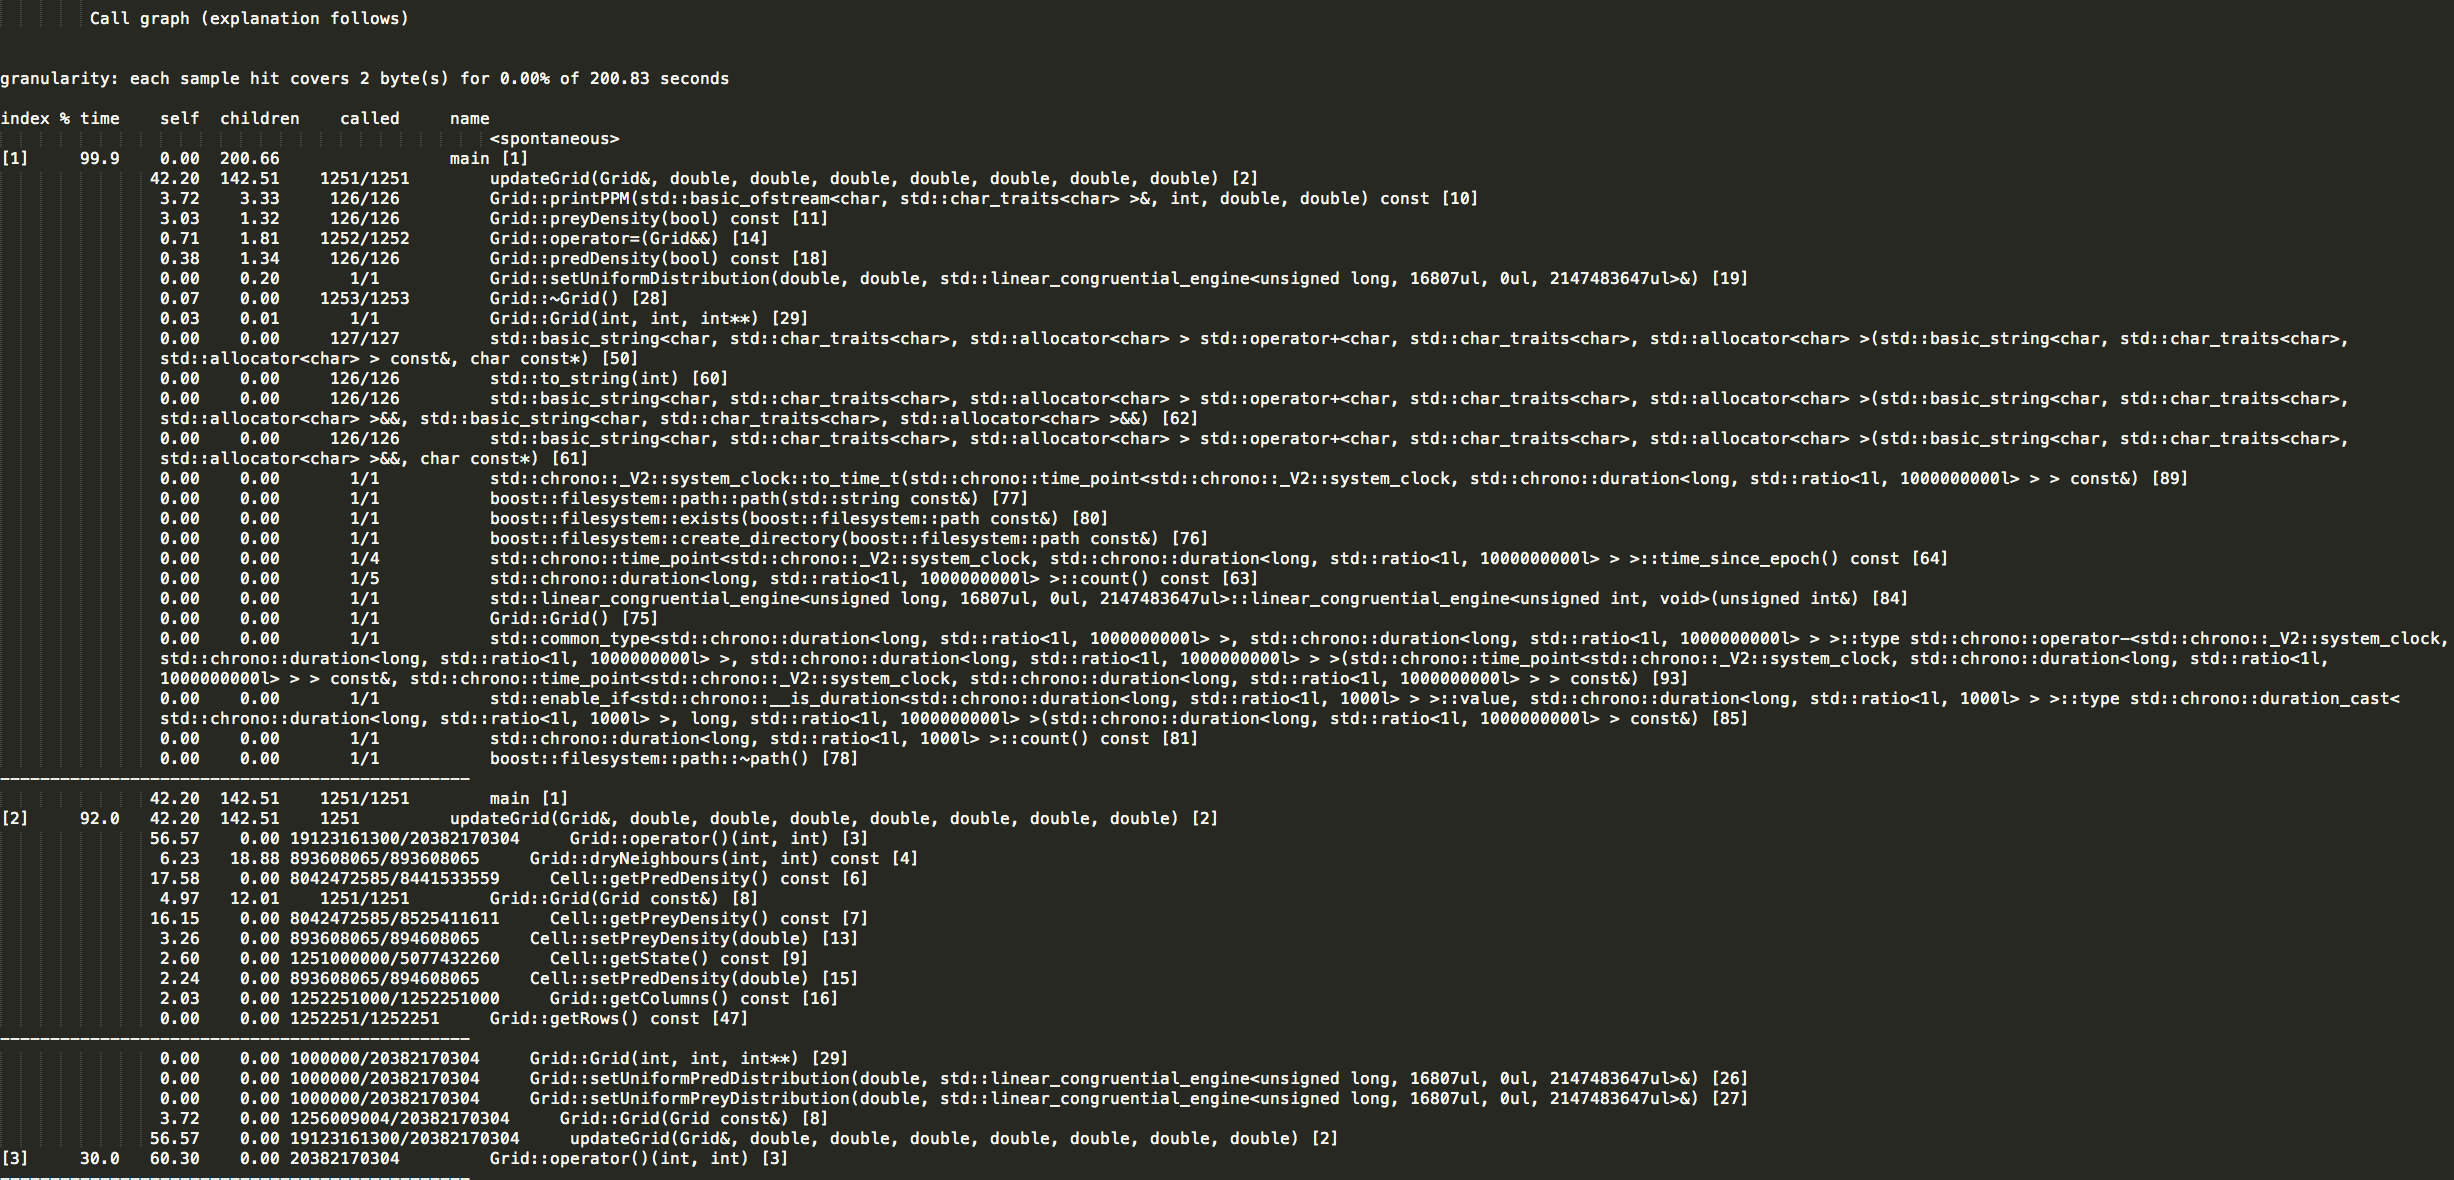
\includegraphics[scale=0.3]{Call-Graph-1.png}}
\caption{Call graph page 1. for Gnu gprof profiler.}
\end{figure}

The \textit{flat profile} shows the total amount of time the program spent executing each function. From \ref{fig:FlatP} we can see the program spent the most time executing the operator(). This is to be expected since the operator() function is used as a utility for accessing the landscape cells in the form (i,j). Due to the fact that internally the landscape is implemented as a 1-D array this function was introduced to make working with the landscape simple and intuitive, and any time access to the landscape is required in the program, the operator() will have been used. One way to reduce the number of function calls to operator() would be to access the elements of the landscape directly in the code using the operator[] on the array of cells. This would make the code for the various Grid methods significantly harder to write and read since all instances of operator(i,j) would become operator[[i + (rows + 1 - j) * (columns+2)]]. An alternative would be to implement the landscape as a 2D array, then the access would be implemented via operator[i][j], however it is likely the overhead of dynamically allocating a 2D array of a user defined type would outweigh the cost of the function we currently have. \\

The \textit{call graph} shows how much time was spent in each function and its children. Form this information we are able to identify functions that themselves do not use much time, but call other functions that use exceptional amounts of time. From \ref{fig:CallG} line [2] we can see that 92\% of the time was spent in the function updateGrid() and its subroutines, which is to be expected since this is the function that evolves the landscape and apart from printing output, most the remaining functions called from the main method perform one off tasks such as setting up initial conditions. Of the function calls from within updateGrid() we can see that operator() clocks in the highest with 56.57s spent within it when it is called from updateGrid(). This supports our above analysis that the function operator() is a serious overhead. From [3] and [5] (not shown in \ref{fig:CallG}) we can see that 39.5\% of the total time is spent in operator() or its constant equivalent. We can also see that it is the methods of the Grid class and the updateGrid() functions that call the operator(). Based on this analysis it would be a good idea to test giving these functions direct access to the grid cells through the operator[] instead of using the overloaded operator(). It may be that moving the functionality from operator() to operator[] means that the functions that call it inherit the overhead instead, however it is worth checking as a possible optimization. 




\subsection{Effects of Input/Output}
\label{subsec:input}

\subsection{subsec:outfreq}
To begin the investigation into the effects of input we vary the number of time steps between the output of the plain .ppm files. The other input parameters are kept fixed at the same values as in section \ref{subsec:opflags}, however the number of steps between the output of the plain .ppm files is varied from 10 to 100 at intervals of 10 steps. The input landscape \ref{fig:OptLandscape} was used for the same reasons as in \ref{subsec:opflags}. Since the program was shown to run fastest when compiled under the -O2 flag in section \ref{subsec:opflags} we have used that option. 

\subsubsection{Landscape Water vs. Land}
\label{subsub:watervsland}

\subsubsection{Landscape Size}
\label{subsub:landscapesize}

\section{Conclusion}
\label{sec:conclusion}

\begin{appendices}
\section{Complete Data Sets}


% Please add the following required packages to your document preamble:
% \usepackage{multirow}
\begin{table}[!h]
\centering
\label{tab:completeOP}
\begin{tabular}{| c | c | c | c | c | c | c |}
\hline
{\textbf{Compiler} & \multicolumn{6}{| c |}{\textbf{Run Time(s)}}                  \\
\cline{2-7}

                          & O0      & O1       & O2        & O3       & Ofast    & Os       \\
                          \hline
      & 247.042 & 181.057 & 171.405  & 171.405 & 177.838 & 190.849 \\
                          & 247.466 & 181.326 & 171.641  & 175.660 & 176.470 & 190.547 \\
 gcc                         & 247.391 & 183.946 & 176.876   & 177.094 & 181.324 & 191.942 \\
                          & 250.712 & 182.675 & 171.137 & 175.355 & 179.191 & 190.994 \\
                          & 250.511 & 180.602 & 171.369  & 174.871 & 174.351 & 188.759 \\
                          & 250.888 & 180.273  & 171.561   & 175.481  & 174.350  & 189.081\\ \hline
\end{tabular}
\caption{Complete data set for gcc optimisation tests on cp lab.}
\end{table}



\begin{table}[!h]
\centering
\label{tab:otsdata}
\begin{tabular}{| c | c | c | c | c | c | c |}
\hline
{\textbf{Number steps} & \multicolumn{6}{| c |}{\textbf{Run Time(s)}}                  \\
\hline
10    & 171.405 & 171.641 & 176.876  & 171.137 & 171.369 & 171.561 \\
\hline
20   & 122.466 & 122.400 & 123.026  & 122.703 & 123.573 & 122.341 \\
\hline
30 & 106.718 & 106.978 & 106.254   & 106.518 & 106.862 & 107.034 \\
\hline
40    & 100.035 & 98.694 & 98.721 & 101.000 & 98.802 & 99.043 \\
\hline
50    & 94.207 & 94.208 & 93.995  & 94.274 & 94.611 & 95.233 \\
\hline
60    & 90.761 & 90.289  & 90.335   & 90.298  & 90.570  & 90.307\\
\hline
70    & 89.597 & 89.076  & 91.979   & 89.224  & 90.130  & 89662\\
\hline
80    & 88.188 & 87.924  & 86.422   & 87.013  & 86.457  & 86.422\\
\hline
90    & 84.877 & 84.799  & 84.838   & 84.877  & 84.945  & 85.100\\
\hline
100    & 84.151 & 84.138  & 84.095   & 84.392  & 84.051  & 84.146\\
\hline
\end{tabular}
\caption{Complete data set for varying number of steps between output of plain .ppm.}
\end{table}


\section{Statistical Equations and Calculations}
Our data sets were small due to the fact jobs had to be submitted individually to stop them slowing each other down. Because of this, we choose to use the \textbf{corrected sample standard deviation} given by:\tabularnewline
\begin{equation}\tabularnewline
\label{eqn:std}
s=\sqrt{\frac{1}{N-1}\sum^{N}_{i=1}(x_i-\bar{x})^2}
\end{equation}
which compensates for the bias in standard deviation which occurs for a small data set. The \textbf{standard error} was then estimated in the usual way using:
\begin{equation}
\label{eqn:stderr}
\sigma_x\approx\frac{s}{\sqrt{N}}
\end{equation}


\end{appendices}





\end{document}